\documentclass[aspectratio=169,11pt]{beamer}
% ==========================================================================
%  KSA lecture-slide theme  =  stock beamer "Boadilla"  +  KSA colour theme
%  brand colours sampled from the official KSA symbol mark:
%    Deep Prussian Blue  #2E3192   (지성 - intellect)
%    Golden Gray         #D6CBB1   (감성 - sensibility)
%  Engine: XeLaTeX.  Usage:
%    \documentclass[aspectratio=169,11pt]{beamer}
%    \input{../../theme/ksa-theme.tex}
%  Each deck lives in its own slides/kor/<deck>/ folder together with its
%  own images; ../../figs/ is kept only as a fallback for the shared cache.
% ==========================================================================

\usepackage{fontspec}
\usepackage{amsmath,amssymb}
\usepackage{graphicx}
\graphicspath{{figs/}{./}{../../../figs/}}
\usepackage{booktabs}
\usepackage{listings}
\usepackage{varwidth}

% ---- fonts (no ctex/xeCJK on this box -> fontspec drives CJK directly) -----
\defaultfontfeatures{Ligatures=TeX}
\setmainfont{Noto Sans CJK KR}
\setsansfont{Noto Sans CJK KR}
\setmonofont{Noto Sans Mono CJK KR}[Scale=0.92]

% ---- base theme: stock Boadilla ------------------------------------------
\usetheme{Boadilla}
\usefonttheme{professionalfonts}
\setbeamertemplate{navigation symbols}{}

% ---- KSA colour theme (recolour the stock theme) --------------------------
\definecolor{ksablue}{HTML}{2E3192}
\definecolor{ksabluedk}{HTML}{20226A}
\definecolor{ksagold}{HTML}{D6CBB1}
\definecolor{ksagolddk}{HTML}{A9976B}
\definecolor{ksared}{HTML}{C0392B}
\definecolor{ksagray}{HTML}{5B5B5B}

\setbeamercolor{structure}{fg=ksablue}
\setbeamercolor{alerted text}{fg=ksared}

\setbeamercolor{palette primary}{fg=white,           bg=ksablue}
\setbeamercolor{palette secondary}{fg=white,         bg=ksablue!85!black}
\setbeamercolor{palette tertiary}{fg=white,          bg=ksabluedk}
\setbeamercolor{titlelike}{fg=ksablue}
\setbeamercolor{frametitle}{fg=ksablue,bg=}
\setbeamercolor{title}{fg=ksablue}
\setbeamercolor{author}{fg=ksagray}
\setbeamercolor{institute}{fg=ksagray}
\setbeamercolor{block title}{fg=white,bg=ksablue}
\setbeamercolor{block body}{fg=black!85,bg=ksablue!6}
\setbeamercolor{item}{fg=ksablue}
\setbeamercolor{section in toc}{fg=black!85}

\setbeamerfont{frametitle}{series=\bfseries}
\setbeamerfont{title}{series=\bfseries}

% ---- footline:  KSA mark | "Made by ..." | n / N   (matches reference) ----
\newcommand{\ksacredit}{}
\setbeamertemplate{footline}{%
  \hbox{%
    \begin{beamercolorbox}[wd=.18\paperwidth,ht=2.6ex,dp=1.5ex,leftskip=1.1em]{}%
      \raisebox{-0.35ex}{\includegraphics[height=2.0ex]{ksa-logo.png}}%
    \end{beamercolorbox}%
    \begin{beamercolorbox}[wd=.64\paperwidth,ht=2.6ex,dp=1.5ex,center]{}%
      {\scriptsize\color{ksagray}\ksacredit}%
    \end{beamercolorbox}%
    \begin{beamercolorbox}[wd=.18\paperwidth,ht=2.6ex,dp=1.5ex,rightskip=1.1em]{}%
      \hfill{\scriptsize\color{ksablue}\insertframenumber\,/\,\inserttotalframenumber}%
    \end{beamercolorbox}%
  }%
  \vskip2pt
}

% ---- section divider: stock \sectionpage, KSA-coloured -------------------
\setbeamertemplate{section page}{%
  \begingroup\centering
    {\color{ksagolddk}\rule{0.16\paperwidth}{1pt}}\par\vskip1.0em
    {\usebeamerfont{title}\color{ksablue}\insertsectionhead\par}\vskip1.0em
    {\color{ksagolddk}\rule{0.16\paperwidth}{1pt}}\par
  \endgroup
}
\AtBeginSection[]{\begin{frame}[plain,noframenumbering]\vfill\sectionpage\vfill\end{frame}}

% ---- code listings ------------------------------------------------------------
\lstdefinestyle{ksa}{%
  basicstyle=\ttfamily\scriptsize,
  keywordstyle=\color{ksablue}\bfseries,
  commentstyle=\color{ksagray}\itshape,
  stringstyle=\color{ksagolddk},
  numberstyle=\tiny\color{ksagray},
  backgroundcolor=\color{ksablue!6},
  frame=leftline, framerule=1.4pt, rulecolor=\color{ksablue},
  xleftmargin=1em, aboveskip=0.8em, belowskip=0.4em,
  showstringspaces=false, breaklines=true, language=Python,
}
\lstset{style=ksa}

% ---- handy macros -----------------------------------------------------------
\newcommand{\kb}[1]{\textbf{\color{ksablue}#1}}   % blue keyword
\newcommand{\kq}[1]{\textbf{\color{ksared}#1}}    % red key-question

\setbeamerfont{title}{series=\bfseries,size=\fontsize{24}{30}\selectfont}
\setbeamerfont{subtitle}{series=\bfseries,size=\fontsize{14}{18}\selectfont}
\setbeamerfont{author}{size=\normalsize}
\setbeamerfont{institute}{size=\small}
\graphicspath{{figs/}{../../../../assets/}}
\makeatletter
\newcommand{\markpage}[1]{\protected@write\@auxout{}{\string\newlabel{#1}{{\the\c@framenumber}{}}}\hypertarget{#1}{}}
\newcommand{\pref}[1]{\hyperlink{#1}{\textcolor{ksagolddk}{(p.\ref{#1})}}}
\makeatother

\renewcommand{\ksacredit}{Machine Learning 1 \,\textperiodcentered\, XOR과 역전파}
\title{XOR 과 역전파 (Backpropagation)}
\subtitle{AI 를 얼어붙게 한 문제, 그리고 숨은 층을 학습하는 방법}
\author{Machine Learning 1}
\institute{한국과학영재학교 (KSA)}
\date{}
\begin{document}
\begin{frame}[plain,noframenumbering]\titlepage\end{frame}

% --- 오늘의 질문
\begin{frame}{오늘의 질문: 직선 하나로 가를 수 있을까?}
\vfill
\centering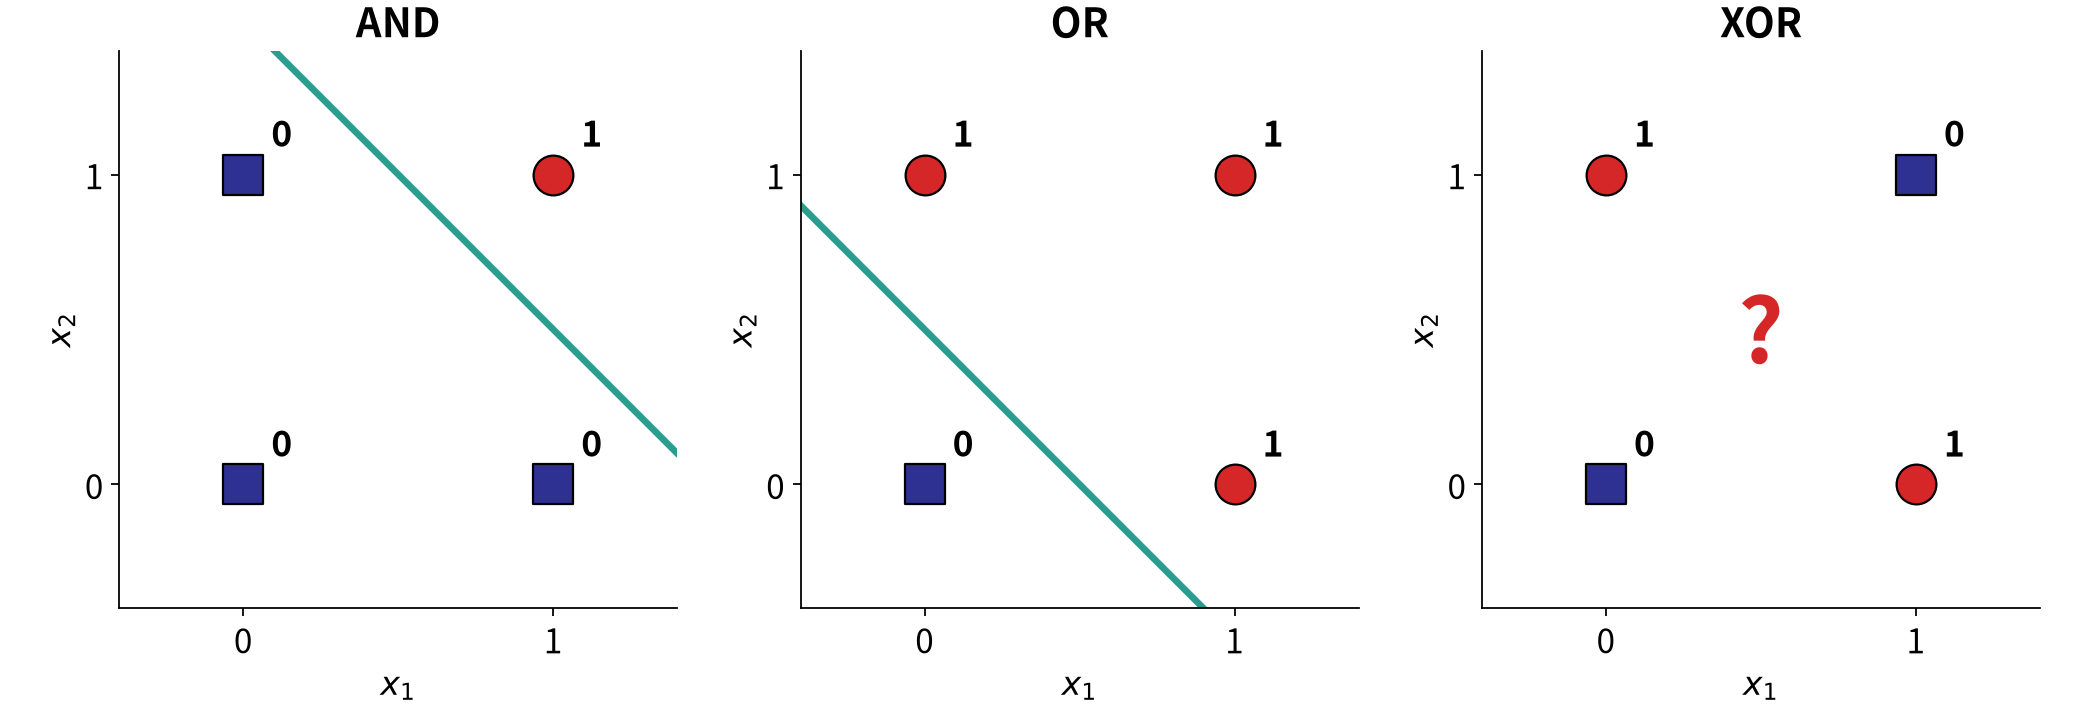
\includegraphics[width=0.9\linewidth]{xo_gates.png}\par\vskip0.2em
{\large AND, OR 는 직선 하나로 가른다 \quad \kq{XOR (두 입력이 다를 때만 1) 은?}}
\vfill
\note{입력 두 개가 0 또는 1인 네 가지 경우입니다. AND는 둘 다 1일 때만 1이고, OR는 하나라도 1이면 1입니다. 둘 다 초록 직선 하나로 1과 0을 가를 수 있습니다. 그러면 XOR은 어떨까요? XOR은 두 입력이 다를 때만 1입니다. 빨간 동그라미 두 개가 대각선으로, 파란 네모 두 개가 다른 대각선으로 놓여 있습니다. 직선 하나를 아무리 돌려 봐도 둘을 가를 수 없습니다. 이 간단한 문제가 한때 인공지능 연구를 얼어붙게 만들었습니다.}
\end{frame}

% --- 퍼셉트론
\begin{frame}{퍼셉트론 (1958): 직선 하나로 분류하는 기계}
\vfill
\centering
{\LARGE\[ y = \begin{cases} 1 & w_1 x_1 + w_2 x_2 + b > 0\\ 0 & \text{otherwise} \end{cases} \]}\vskip0.4em
{\large F. Rosenblatt 가 만든 첫 학습하는 신경망 \quad 경계 $w_1 x_1 + w_2 x_2 + b = 0$ 은 \textbf{직선}}\\[0.6em]
{\large OR: \; $w = (1, 1)$, $b = -0.5$ \qquad AND: \; $w = (1, 1)$, $b = -1.5$}\\[0.6em]
{\small 지금 신경망의 뉴런 하나와 같다 (계단 대신 시그모이드 · ReLU 를 쓸 뿐)}
\vfill
\note{1958년 로젠블랫은 퍼셉트론이라는 학습하는 기계를 만들었습니다. 입력에 가중치를 곱해 더하고 b를 더한 값이 0보다 크면 1, 아니면 0을 냅니다. 경계인 w1 x1 더하기 w2 x2 더하기 b가 0인 곳은 직선입니다. 2주차 로지스틱회귀의 경계가 직선이었던 것과 같습니다. OR는 가중치 1, 1에 b를 마이너스 0.5로, AND는 b를 마이너스 1.5로 두면 됩니다. 지금 신경망의 뉴런 하나가 바로 이 퍼셉트론이고, 계단 함수 대신 시그모이드나 ReLU를 쓸 뿐입니다.}
\end{frame}

% --- XOR 불가능
\begin{frame}{XOR 은 왜 직선 하나로 안 되나}
\vfill
\centering
{\large 직선 하나로 된다고 해 보자: \quad $w_1 x_1 + w_2 x_2 + b$}\vskip0.5em
\renewcommand{\arraystretch}{1.3}
{\Large\begin{tabular}{lll}
$(0, 0) \to 0$ & $b \le 0$ & \\
$(0, 1) \to 1$ & $w_2 + b > 0$ & \\
$(1, 0) \to 1$ & $w_1 + b > 0$ & \\
$(1, 1) \to 0$ & $w_1 + w_2 + b \le 0$ &
\end{tabular}}\vskip0.5em
{\large 가운데 두 줄의 합 $w_1 + w_2 + 2b > 0$ 에 $-b \ge 0$ 을 더하면 $w_1 + w_2 + b > 0$ \quad \kq{넷째 줄과 모순}}
\vfill
\note{XOR이 직선 하나로 안 된다는 걸 증명해 봅시다. 된다고 가정하면 네 점마다 조건이 하나씩 생깁니다. (0, 0)은 0이어야 하니 b가 0 이하, (0, 1)과 (1, 0)은 1이어야 하니 w2 더하기 b와 w1 더하기 b가 양수, (1, 1)은 0이어야 하니 w1 더하기 w2 더하기 b가 0 이하입니다. 가운데 두 부등식을 더하면 w1 더하기 w2 더하기 2b가 양수이고, 여기에 첫 줄에서 얻은 마이너스 b가 0 이상이라는 걸 더하면 w1 더하기 w2 더하기 b가 양수입니다. 넷째 줄과 모순입니다. 어떤 가중치로도 안 됩니다.}
\end{frame}

% --- 역사
\begin{frame}{1969년, 신경망의 겨울}
\vfill
\centering
\renewcommand{\arraystretch}{1.6}
{\large\begin{tabular}{rl}
1958 & 로젠블랫의 퍼셉트론, 큰 기대\\
1969 & 민스키 \& 페퍼트 《Perceptrons》: 한 층의 한계 (XOR 등)\\
1970 $\sim$ 80년대 중반 & 연구비 · 관심이 크게 준다 (약 15년의 \kq{겨울})\\
1986 & 루멜하트 · 힌턴 · 윌리엄스: \textbf{역전파} (\textit{Nature})
\end{tabular}}\vskip0.8em
{\small 층을 쌓으면 XOR 이 풀린다는 건 알려져 있었다. 문제는 숨은 층을 \textbf{학습}하는 방법이었다}
\vfill
\note{역사를 잠깐 봅니다. 1958년 퍼셉트론은 큰 기대를 받았습니다. 그런데 1969년 민스키와 페퍼트가 Perceptrons라는 책에서 한 층짜리 퍼셉트론이 XOR 같은 간단한 문제도 풀지 못한다는 한계를 수학적으로 정리했습니다. 이후 1970년대부터 1980년대 중반까지 약 15년간 신경망 연구비와 관심이 크게 줄었습니다. 이 시기를 신경망의 겨울이라고 부릅니다. 사실 층을 여러 개 쌓으면 XOR을 풀 수 있다는 건 알려져 있었습니다. 문제는 그 숨은 층의 가중치를 데이터로 학습하는 방법이었고, 1986년 역전파가 그 답이 됩니다.}
\end{frame}

% --- 층을 쌓으면
\begin{frame}{층을 쌓으면: 직선 두 개를 조합한다}
\markpage{two}
\vfill
\centering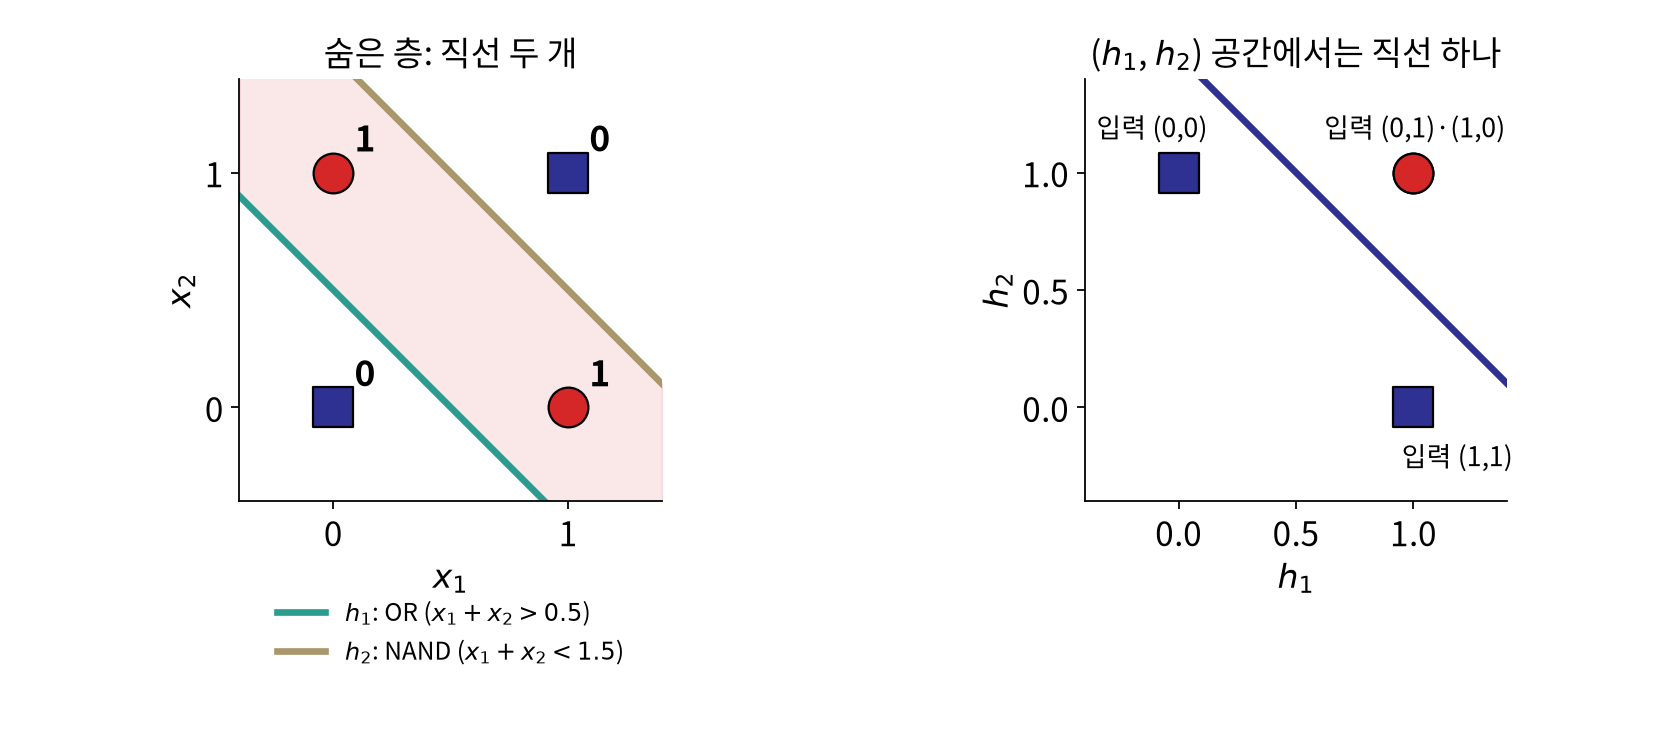
\includegraphics[width=0.74\linewidth]{xo_twolines.png}\par\vskip0.1em
{\large $h_1 = $ OR, \; $h_2 = $ NAND, \; $y = $ AND$(h_1, h_2)$ \quad 숨은 층이 \kb{직선 하나로 갈리게} 만든다}
\vfill
\note{층을 하나 더 쌓아 봅니다. 숨은 뉴런 h1은 OR, 즉 x1 더하기 x2가 0.5보다 크면 1입니다. h2는 NAND, x1 더하기 x2가 1.5보다 작으면 1입니다. 두 직선 사이 띠가 XOR의 1인 영역입니다. 오른쪽은 네 입력을 h1, h2 공간으로 옮긴 그림입니다. (0, 1)과 (1, 0)은 둘 다 (1, 1)로 모이고, (0, 0)은 (0, 1), (1, 1)은 (1, 0)으로 갑니다. 이 공간에서는 파란 직선 하나로 가를 수 있습니다. 출력 뉴런은 h1과 h2의 AND입니다. 숨은 층이 공간을 바꿔서 직선으로 갈리게 만든 겁니다. 이 생각이 딥러닝 전체의 핵심입니다.}
\end{frame}

% --- 신경망 식
\begin{frame}{2-2-1 신경망}
\vfill
\centering
{\LARGE\[ \mathbf{h} = \sigma(\mathbf{x} W_1 + \mathbf{b}_1) \qquad y = \sigma(\mathbf{h}\cdot\mathbf{w}_2 + b_2) \]}\vskip0.4em
\renewcommand{\arraystretch}{1.3}
{\large\begin{tabular}{ll}
$\mathbf{x}$ & 입력 2개 \quad $\to$ \quad $W_1$ ($2 \times 2$), $\mathbf{b}_1$: 숨은 층\\
$\mathbf{h}$ & 숨은 뉴런 2개 \quad $\to$ \quad $\mathbf{w}_2$ (2개), $b_2$: 출력층\\
$\sigma$ & 시그모이드 (계단 대신 미분할 수 있게)\\
$L = \frac12 (y - t)^2$ & 정답 $t$ 와의 오차
\end{tabular}}\vskip0.4em
{\large 손으로 고른 가중치 대신, 가중치 \textbf{9개}를 데이터로 학습하고 싶다}
\vfill
\note{식으로 쓰면, 입력 x에 가중치 행렬 W1을 곱하고 b1을 더해 시그모이드를 씌운 것이 숨은 층 h입니다. h에 w2를 곱하고 b2를 더해 시그모이드를 씌운 것이 출력 y입니다. 계단 함수 대신 시그모이드를 쓰는 이유는 미분할 수 있어야 경사하강법을 쓸 수 있기 때문입니다. 오차는 정답 t와의 차이 제곱의 절반입니다. 앞 쪽에서는 가중치를 손으로 골랐지만, 이제 W1의 4개, b1의 2개, w2의 2개, b2의 1개, 모두 9개를 데이터로 학습하고 싶습니다.}
\end{frame}

% --- 문제
\begin{frame}{문제: 숨은 층의 가중치는 어떻게 고치나?}
\vfill
\centering
{\large 출력층 $\mathbf{w}_2$: 오차가 바로 보인다 (선형회귀 · 로지스틱회귀처럼)}\\[0.8em]
{\large 숨은 층 $W_1$: 정답이 없다. \kq{$h_1$ 이 얼마여야 했는지} 아무도 모른다}\\[1.0em]
{\LARGE\[ \frac{\partial L}{\partial W_1} = ? \]}\vskip0.4em
{\large 답: $W_1 \to \mathbf{h} \to y \to L$ 로 이어진 \textbf{연쇄법칙}을 거꾸로 따라간다 = \kb{역전파}}
\vfill
\note{출력층의 가중치 w2는 고치기 쉽습니다. 출력 y와 정답 t의 차이가 바로 보이니까 2주차 로지스틱회귀처럼 하면 됩니다. 문제는 숨은 층입니다. 숨은 뉴런 h1이 원래 얼마여야 했는지에 대한 정답은 데이터에 없습니다. 그러면 W1을 어느 방향으로 고쳐야 오차가 줄어들까요? 답은 W1이 h를 바꾸고, h가 y를 바꾸고, y가 L을 바꾸는 사슬을 따라 미분하는 겁니다. 연쇄법칙을 출력에서 입력 쪽으로 거꾸로 따라가는 방법, 역전파입니다.}
\end{frame}

% --- 출력층
\begin{frame}{역전파 1: 출력층}
\markpage{out}
\vfill
\centering
{\LARGE\[ \frac{\partial L}{\partial \mathbf{w}_2} = \underbrace{(y - t)}_{\partial L / \partial y}\;\underbrace{y(1-y)}_{\partial y / \partial z_2}\;\underbrace{\mathbf{h}}_{\partial z_2 / \partial \mathbf{w}_2} = \delta_2\,\mathbf{h} \]}\vskip0.4em
{\large $\delta_2 = (y - t)\,y(1-y)$: 출력의 \textbf{오차 신호}}\\[0.4em]
{\small 시그모이드의 미분: $\sigma'(z) = \sigma(z)(1 - \sigma(z))$ \qquad $z_2 = \mathbf{h}\cdot\mathbf{w}_2 + b_2$}
\vfill
\note{먼저 출력층입니다. 손실 L을 w2로 미분하면 연쇄법칙으로 세 개의 곱이 됩니다. L을 y로 미분하면 y 빼기 t, y를 그 안의 z2로 미분하면 시그모이드의 미분인 y 곱하기 1 빼기 y, z2를 w2로 미분하면 h입니다. 앞의 두 개를 묶어 델타2라고 부르겠습니다. 출력 쪽의 오차 신호입니다. 그러면 w2의 기울기는 델타2 곱하기 h, 오차 신호 곱하기 그 가중치로 들어온 입력입니다. 선형회귀의 기울기가 오차 곱하기 입력이었던 것과 같은 모양입니다.}
\end{frame}

% --- 숨은 층
\begin{frame}{역전파 2: 숨은 층으로 거꾸로}
\markpage{hidden}
\vfill
\centering
{\LARGE\[ \delta_1 = \delta_2\,\mathbf{w}_2 \odot \mathbf{h}(1-\mathbf{h}) \qquad \frac{\partial L}{\partial W_1} = \mathbf{x}^\top \delta_1 \]}\vskip0.6em
{\large 출력의 오차 신호 $\delta_2$ 를 \textbf{그 길의 가중치 $\mathbf{w}_2$ 만큼 나눠} 숨은 뉴런에 돌려보낸다}\\[0.4em]
{\large 숨은 뉴런마다 자기 시그모이드의 기울기를 곱하면 $\delta_1$ \quad 그다음은 출력층과 같은 모양}\\[0.6em]
{\small $\odot$: 칸별 곱 \qquad 층이 더 있어도 같은 일을 반복한다}
\vfill
\note{이제 숨은 층입니다. 숨은 뉴런 h가 y에 영향을 준 정도는 w2입니다. 그래서 출력의 오차 신호 델타2를 w2만큼 나눠서 각 숨은 뉴런에게 돌려보냅니다. 출력에 크게 기여한 뉴런일수록 책임도 크게 받습니다. 여기에 숨은 뉴런 자신의 시그모이드 기울기 h 곱하기 1 빼기 h를 곱하면 숨은 층의 오차 신호 델타1이 됩니다. 그다음은 출력층과 같습니다. W1의 기울기는 입력 x 곱하기 델타1입니다. 층이 10개, 100개여도 이 일을 출력에서 입력 쪽으로 한 층씩 반복하면 됩니다. 정답이 없던 숨은 층에 오차 신호를 만들어 준 것이 역전파의 핵심입니다.}
\end{frame}

% --- 손 계산
\begin{frame}{손으로 한 번}
\markpage{hand}
\vfill
\centering
{\large 입력 $(1, 1)$, 정답 $t = 0$ \quad $W_1 = \begin{bmatrix}1 & -1\\ 1 & -1\end{bmatrix}$, \; $\mathbf{w}_2 = (1, 1)$, \; 편향 0}\vskip0.4em
\renewcommand{\arraystretch}{1.35}
{\large\begin{tabular}{lll}
\textbf{순전파} & $\mathbf{z}_1 = (2, -2)$, \; $\mathbf{h} = (0.881, 0.119)$ & $y = 0.731$, \; $L = 0.267$\\
\textbf{출력층} & $\delta_2 = 0.731 \cdot 0.731 \cdot 0.269 = \kb{0.144}$ & $\partial L / \partial \mathbf{w}_2 = (0.127, 0.017)$\\
\textbf{숨은 층} & $\delta_1 = 0.144 \cdot 1 \cdot 0.105 = \kb{0.015}$ & $\partial L / \partial W_1$: 모든 칸 0.015
\end{tabular}}\vskip0.5em
{\large 경사하강: 가중치를 기울기 반대로 \quad $\to$ $y$ 가 정답 0 쪽으로 내려간다}
\vfill
\note{작은 숫자로 한 번 해 봅니다. 입력 (1, 1), 정답 0입니다. 순전파부터 하면 z1은 (2, 마이너스 2), 시그모이드를 씌우면 h는 0.881과 0.119, 출력 z2는 둘을 더한 1.0, y는 0.731입니다. 정답은 0인데 0.731이니 손실은 0.267입니다. 출력층의 오차 신호 델타2는 0.731 곱하기 0.731 곱하기 0.269, 0.144입니다. w2의 기울기는 이걸 h에 곱한 0.127과 0.017입니다. 숨은 층은 델타2에 w2 1을 곱하고 h 곱하기 1 빼기 h, 0.105를 곱해 0.015입니다. 두 숨은 뉴런이 대칭이라 같습니다. W1의 기울기는 모든 칸 0.015입니다. 가중치를 이 반대로 움직이면 y가 정답 0 쪽으로 내려갑니다.}
\end{frame}

% --- 학습
\begin{frame}{XOR 학습: 정확도 50\% $\to$ 100\%}
\vfill
\centering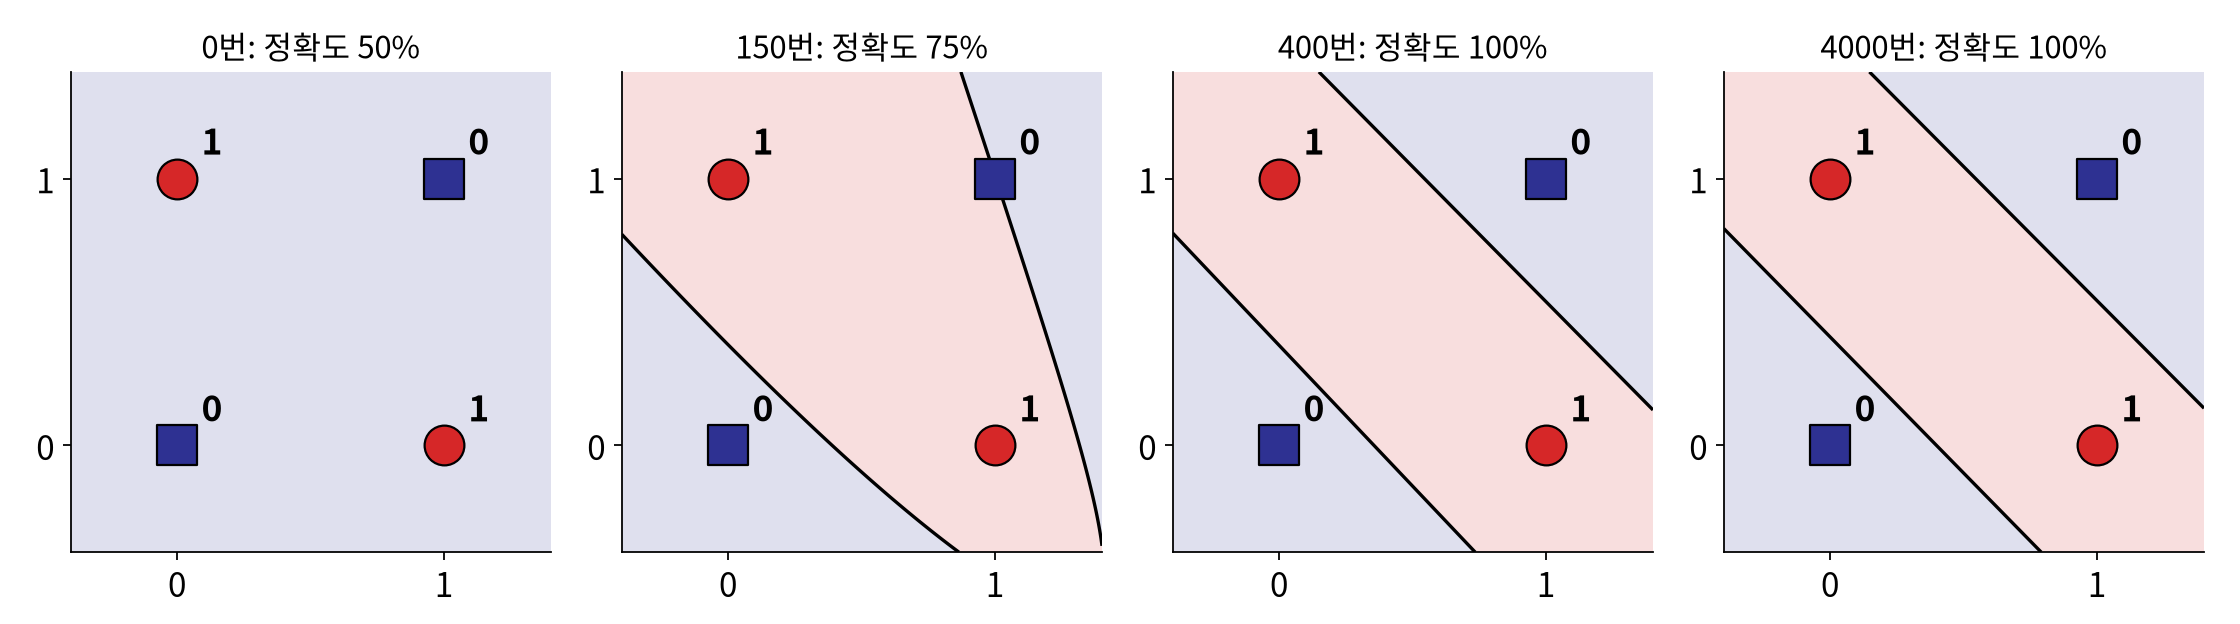
\includegraphics[width=0.96\linewidth]{xo_train.png}\par\vskip0.2em
{\large 학습률 2.0 \quad 150번 75\% \quad 400번 \kb{100\%} \quad 4,000번: 0.012 · 0.986 · 0.986 · 0.013}
\vfill
\note{네 점 전체로 역전파와 경사하강법을 반복했습니다. 무작위 가중치에서 시작하면 처음에는 모든 점에 0.4 근처를 내서 정확도 50퍼센트입니다. 150번째에는 경계가 하나 생겨 75퍼센트, 400번째에는 두 경계가 생기며 100퍼센트가 됩니다. 4000번 뒤 출력은 0.012, 0.986, 0.986, 0.013으로 정답 0, 1, 1, 0에 아주 가깝습니다. 손으로 고르지 않은 숨은 층이 스스로 직선 두 개를 찾아냈습니다.}
\end{frame}

% --- 의미
\begin{frame}{역전파가 연 길}
\vfill
\centering
\renewcommand{\arraystretch}{1.5}
{\large\begin{tabular}{ll}
1986 & 여러 층 신경망을 학습할 수 있게 됐다\\
오늘 & 층 수백 개, 가중치 수십억 개도 \textbf{같은 원리}\\
PyTorch & \texttt{loss.backward()} 한 줄이 역전파 (계산 그래프를 거꾸로)
\end{tabular}}\vskip0.8em
{\large 그런데 층을 깊게 쌓자 새로운 문제가 나타났다 $\to$ 다음 시간: \kq{기울기 소실}}
\vfill
\note{1986년 루멜하트, 힌턴, 윌리엄스가 네이처에 역전파로 여러 층 신경망을 학습하는 방법을 발표하면서 신경망의 겨울이 끝나기 시작했습니다. 오늘날 층이 수백 개, 가중치가 수십억 개인 모델도 정확히 같은 원리로 학습합니다. PyTorch에서 loss.backward 한 줄이 바로 오늘 손으로 한 계산을 계산 그래프를 따라 자동으로 해 줍니다. 그런데 층을 아주 깊게 쌓자 새로운 문제가 나타났습니다. 다음 시간에 배울 기울기 소실입니다.}
\end{frame}

% --- 문제풀이
\begin{frame}{문제풀이}
\vfill
\begin{enumerate}
\item NAND (둘 다 1 일 때만 0) 를 퍼셉트론 하나로 만드는 $w_1, w_2, b$ 를 하나 찾아라.\vskip0.8em
\item 손 계산 예 \pref{hand} 에서 정답이 $t = 1$ 이었다면 $\delta_2$ 의 부호는? 가중치는 어느 쪽으로 움직이나?\vskip0.8em
\item 숨은 뉴런의 시그모이드 출력이 $h = 0.99$ 이면 $h(1-h)$ 는? 이 뉴런으로 가는 오차 신호는 어떻게 되나?\vskip0.8em
\item 2-2-1 신경망의 가중치 · 편향은 모두 몇 개인가? 2-3-1 이면?
\end{enumerate}
\vfill
\note{1번 답. 예를 들어 w1, w2를 마이너스 1, b를 1.5로 두면 둘 다 1일 때만 마이너스 0.5로 0이 됩니다. 2번 답. y 빼기 t가 0.731 빼기 1로 음수라 델타2도 음수입니다. 기울기 반대로 가니 가중치가 커지는 쪽, y가 1 쪽으로 올라가게 움직입니다. 3번 답. 0.99 곱하기 0.01, 0.0099로 아주 작아서 이 뉴런으로 가는 오차 신호가 거의 사라집니다. 다음 시간 기울기 소실의 씨앗입니다. 4번 답. 2-2-1은 W1 4개, b1 2개, w2 2개, b2 1개로 9개, 2-3-1은 6 더하기 3 더하기 3 더하기 1, 13개입니다.}
\end{frame}

% --- 실습
\begin{frame}{실습}
\vfill
\centering\begin{tabular}{rl}
\large 1 & numpy 로 2-2-1 신경망 + 역전파 직접 구현 $\to$ XOR 100\%\\[0.5em]
\large 2 & 기울기 확인: 역전파 기울기 vs 숫자로 조금 움직여 본 기울기\\[0.5em]
\large 3 & PyTorch \texttt{loss.backward()} 로 같은 계산 + 실제 손글씨 숫자 분류
\end{tabular}\vskip1em
Optical Recognition of Handwritten Digits (UCI; scikit-learn \texttt{load\_digits}) \\[0.4em]\href{https://colab.research.google.com/github/SuminHan/book-ml/blob/main/slides/v2/ml1/week09/xor_backprop/lab/xor_backprop.ipynb}{\textcolor{ksagolddk}{▶ Colab에서 실습 노트북 열기}}
\vfill
\note{실습은 세 부분입니다. 첫째, numpy로 2-2-1 신경망과 역전파를 직접 구현해서 XOR을 100퍼센트 맞힙니다. 둘째, 역전파로 구한 기울기가 맞는지, 가중치를 아주 조금 움직여 손실이 변한 양으로 구한 숫자 기울기와 비교합니다. 셋째, 같은 계산을 PyTorch의 loss.backward로 해서 값이 같은지 확인하고, 실제 손글씨 숫자 데이터를 분류하는 작은 신경망을 학습합니다.}
\end{frame}

% --- 정리
\begin{frame}{정리}
\vfill
\centering\large\begin{tabular}{l}
퍼셉트론 = 직선 하나 \quad XOR 은 직선 하나로 못 가른다 $\to$ 신경망의 겨울 (1969)\\[0.5em]
숨은 층이 공간을 바꿔 직선으로 갈리게 만든다 (OR · NAND $\to$ AND)\\[0.5em]
\textbf{역전파}: 오차 신호 $\delta$ 를 연쇄법칙으로 출력 $\to$ 입력 쪽으로 돌려보낸다\\[0.5em]
$\partial L / \partial W = $ (들어온 입력) $\times$ (오차 신호) \quad XOR 50\% $\to$ 100\%
\end{tabular}
\vfill
\note{정리합니다. 퍼셉트론은 직선 하나로 분류하는데, XOR은 직선 하나로 가를 수 없고 이것이 1969년 이후 신경망의 겨울로 이어졌습니다. 숨은 층을 쌓으면 공간이 바뀌어 직선으로 가를 수 있게 됩니다. 그 숨은 층을 학습하는 방법이 역전파입니다. 출력의 오차 신호를 연쇄법칙으로 입력 쪽으로 한 층씩 돌려보내고, 각 가중치의 기울기는 들어온 입력 곱하기 오차 신호입니다. 그렇게 XOR을 50퍼센트에서 100퍼센트로 학습했습니다.}
\end{frame}
\end{document}
